\documentclass[11pt]{article}
\usepackage[margin=1in]{geometry}
\usepackage{amsmath,amssymb,booktabs,graphicx,caption,hyperref,siunitx}
\graphicspath{{../}}
\captionsetup{font=small,labelfont=bf}
\newcommand{\rel}{\mathrm{relerr}}
\title{Local-KLE (multiscale) pCN samplers on a Darcy inverse problem:\\ pre-sampling tests and production results}
\author{Aidan Gettemy (study), report drafted with Claude}
\date{3 November 2026}
\begin{document}
\maketitle

\begin{abstract}
We compare six pCN samplers for the log-permeability coefficients of a $32\times32$ Darcy problem (no $\beta$, no $\rho$; squared-exponential prior, $\ell=0.1$, $r=64$ modes): global pCN (1), local-KLE primal raw (2), primal whitened with a pseudo-inverse (3a) and with the null-space term (3b), a primal/dual mixture (4), and a primal$\to$dual sequence (5). Whitening is exact only for the full-rank case; the primal $4\times4$ decomposition with 4 local modes per block has $\operatorname{rank}\Sigma_{ms}=58<64$. Prior tests (likelihood off) and production runs (64 chains, $10^5$ iterations) agree on the ordering of the samplers. \textbf{3b is statistically indistinguishable from global pCN; 3a, 2 and 5 show a modest loss of posterior spread (about 10--17\%); experiment 4 fails in practice} because its primal move is almost never accepted (0.16\%), and its results should not be read as a posterior.
\end{abstract}

\section{Summary of findings}
\begin{enumerate}
\item \textbf{Rank.} The primal $\Sigma_{ms}=BB^\top$ is rank deficient by exactly six directions ($r_+=58$); the dual one is full rank ($r_+=64$, cond $10.7$). Whitening therefore needs either the pseudo-inverse (3a) or the report's null-space term (3b).
\item \textbf{3b reproduces global pCN.} Prior test: covariance error $0.023$ for both. Production: mean posterior sd of $\log\kappa$ $0.575$ vs.\ $0.570$, same acceptance, same relative-error plateau, MPSRF $1.12$ vs.\ $1.13$. It is a correctness device, as predicted, not a speed-up.
\item \textbf{Raw and pseudo-inverse samplers lose spread.} Mean posterior sd of $\log\kappa$ relative to experiment 1: 2: $0.83$, 3a: $0.90$, 5: $0.86$. The ordering matches the prior-test variance deficits (pointwise variance ratios $0.78$, $0.93$, $0.78/0.75$).
\item \textbf{Experiment 4 is not usable as configured.} The primal move's step size sank to its floor ($10^{-3}$) and its acceptance is $0.16\%$; the chains plateau at $\rel=0.033$ (others $0.020$), MPSRF is $1.61$, and the posterior sd collapses to $0.22$ ($0.38\times$ experiment 1).
\item \textbf{All well-behaved samplers plateau at the same relative error, $\rel\approx0.0204$,} about $6.4\times$ the data noise level ($0.0032$), as anticipated by the group; $\Phi\approx 23$ there.
\item \textbf{Experiment 5} switches from primal to dual with essentially no cost: median $\Phi$ $23.6\to24.8$, $\rel$ $0.0206\to0.0211$.
\end{enumerate}
All conclusions rest on one synthetic data set (truth seed 2026) and one set of chain seeds; no repeated-data uncertainty is quantified (Section~\ref{sec:caveats}).

\section{Setup}
\textbf{Problem.} Unit square, $32\times32$ cells ($N=1024$); $\log\kappa=T\theta$, $\theta\sim N(0,I_{64})$ (KLE at energy $0.966$ gives $r=64$, modes 63/64 a tied pair); pressure $1$ on the left and $0$ on the right face, no flow top and bottom (Dirichlet permeameter, harmonic transmissibilities). Data: pressure on 512 checkerboard cells, truth a fixed-seed prior draw, additive Gaussian noise with global relative size $0.003$. Likelihood $\Phi=\|d-Op\|^2/(2\sigma_{rel}^2\|d\|^2)$ with $\sigma_{rel}=0.003$. With this global-norm likelihood the expected $\Phi$ at the truth is $\approx0.5$ (realised $0.567$, $\rel=0.0032$).

\textbf{Samplers.} All use pCN, $s_{\rm new}=\sqrt{1-s^2}\,x+s\xi$, acceptance on the likelihood ratio only, one forward solve per iteration, one step size per grid (all blocks proposed together), adapted to 25\% acceptance for the first $M=10^4$ iterations (each phase for 5) and then frozen. $B$ is the assemble-and-project matrix from local KLE coefficients $c$ to the global KLE.
\begin{center}\small
\resizebox{\textwidth}{!}{\begin{tabular}{@{}lll@{}}\toprule
 & state & $\theta$\\ \midrule
1 & $\theta$ & $\theta$ (global pCN)\\
2 & $c$ (primal, $p=64$) & $Bc$ (raw; prior $N(0,\Sigma_{ms})$)\\
3a & $c$ & $W_+Bc$ (pseudo-inverse; prior $N(0,V_+V_+^\top)$)\\
3b & $(c,\zeta)$, $\zeta\in\mathbb R^6$ & $W_+Bc+V_0\zeta$ (exact $N(0,I)$)\\
4 & $\theta$; w.p.\ $\tfrac12$ each: $c_g=\Pi_g\theta$, pCN step, $\theta'=B_gc'_g$ & primal or dual grid\\
5 & $c$: $K=5\cdot10^4$ primal iterations, then $c=\Pi_{\rm dual}\theta$ and $5\cdot10^4$ dual & raw, $\theta=B_gc$\\ \bottomrule
\end{tabular}}\end{center}
Primal grid: $4\times4$ blocks, 4 local modes each. Dual grid: $5\times5$ tiling with interfaces at $(i+\tfrac12)/4$, block dimensions from the 95\% local-energy rule ($p=114$). Runs: 64 chains, $N=10^5$, $K=5\cdot10^4$, identical seeds across experiments; $\theta$ and local coefficients saved every 100 iterations, relative error and acceptance every iteration. About $103$\,s per chain.

\section{Tests before sampling}
\subsection{\texorpdfstring{$\Sigma_{ms}$}{Sigma\_ms} rank test}
\begin{center}\small
\begin{tabular}{@{}lrrrrl@{}}\toprule
grid & $p$ & $r_+$ (of 64) & $d_{\min}$ & cond$(\Sigma_{ms})$ & result\\ \midrule
primal & 64 & 58 & $-2.9\times10^{-16}$ & $\infty$ & FAIL\\
dual & 114 & 64 & $0.284$ & $10.7$ & PASS\\ \bottomrule
\end{tabular}\end{center}
The primal $B$ ($64\times64$) has a 12-orders-of-magnitude gap in its singular values after the 58th (Fig.~\ref{fig:rank}); an independent MATLAB computation of $G=B^\top B$ agreed (deficient by exactly six). By decision the study proceeds with four modes per block and splits experiment 3 into 3a/3b. Whitening with the null-space term has operator error $6\times10^{-15}$.
\begin{figure}[h]\centering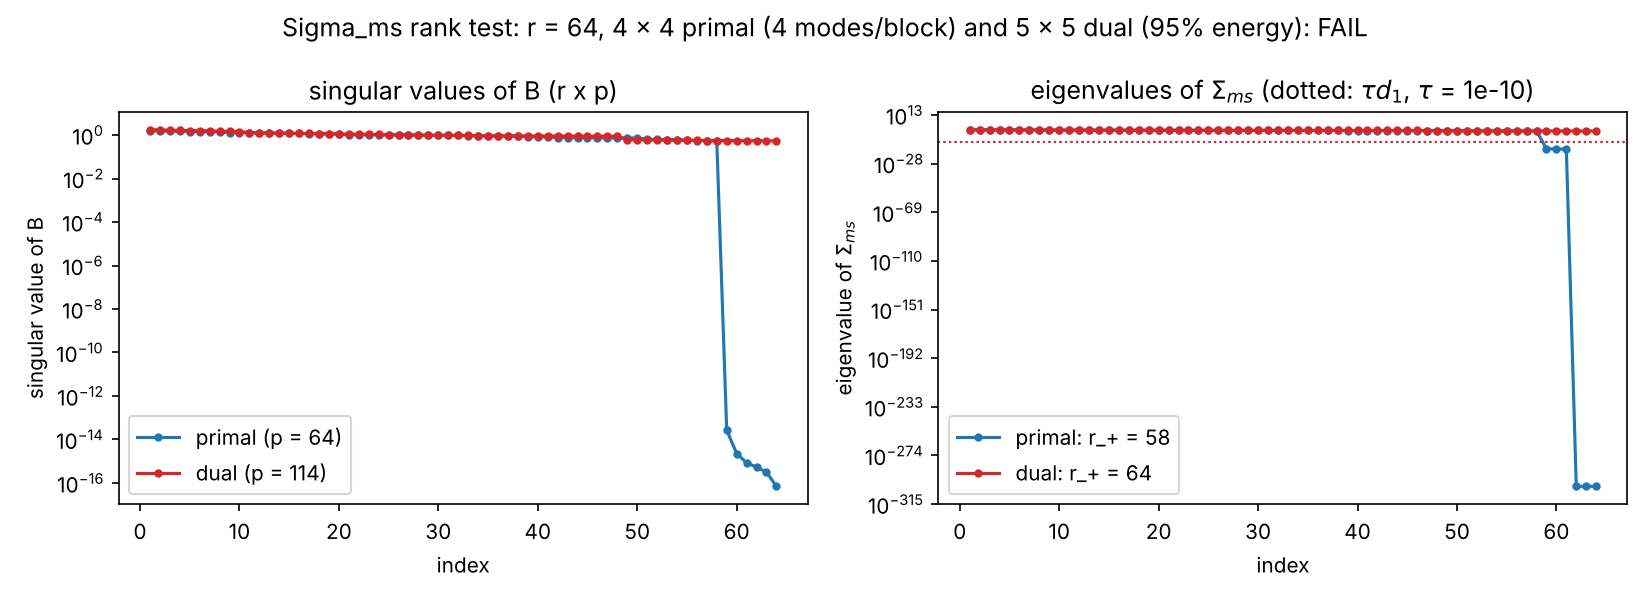
\includegraphics[width=.85\textwidth]{figures/msm_rank_test/fig_msm_rank_test.png}
\caption{Singular values of $B$ and eigenvalues of $\Sigma_{ms}$, primal and dual.}\label{fig:rank}\end{figure}

\subsection{Prior test (likelihood off)}
With $\Phi\equiv0$ every proposal is accepted; the chains should reproduce $N(0,I_{64})$ if the sampler preserves the prior. 64 chains, $4\times10^4$ iterations, $s=0.5$.
\begin{center}\small
\begin{tabular}{@{}lrrr@{}}\toprule
sampler & cov.\ error (Frob/$\sqrt r$) & pointwise var.\ ratio (mean) & range\\ \midrule
reference & 0.022 & 1.000 & 0.99--1.01\\
1 global & 0.023 & 1.000 & 0.99--1.01\\
2 primal raw & 0.631 & 0.783 & 0.31--1.22\\
3a pseudo-inverse & 0.307 & 0.925 & 0.80--1.01\\
3b null-space term & 0.023 & 1.001 & 0.99--1.01\\
4 mixture & 0.422 & 0.619 & 0.51--0.97\\
5 phase 1 / phase 2 & 0.631 / 0.741 & 0.783 / 0.752 & 0.31--1.21 / 0.35--1.32\\ \bottomrule
\end{tabular}\end{center}
3a's error $0.307$ matches the exact value $\sqrt{6/64}=0.306$ for dropping six unit-variance directions. Alternating primal and dual moves (experiment 4) does \emph{not} remove the pointwise variance deficit; it deepens it. The switch in experiment 5 changes the field by $8\%$ (relative $L_2$) on prior draws.
\begin{figure}[h]\centering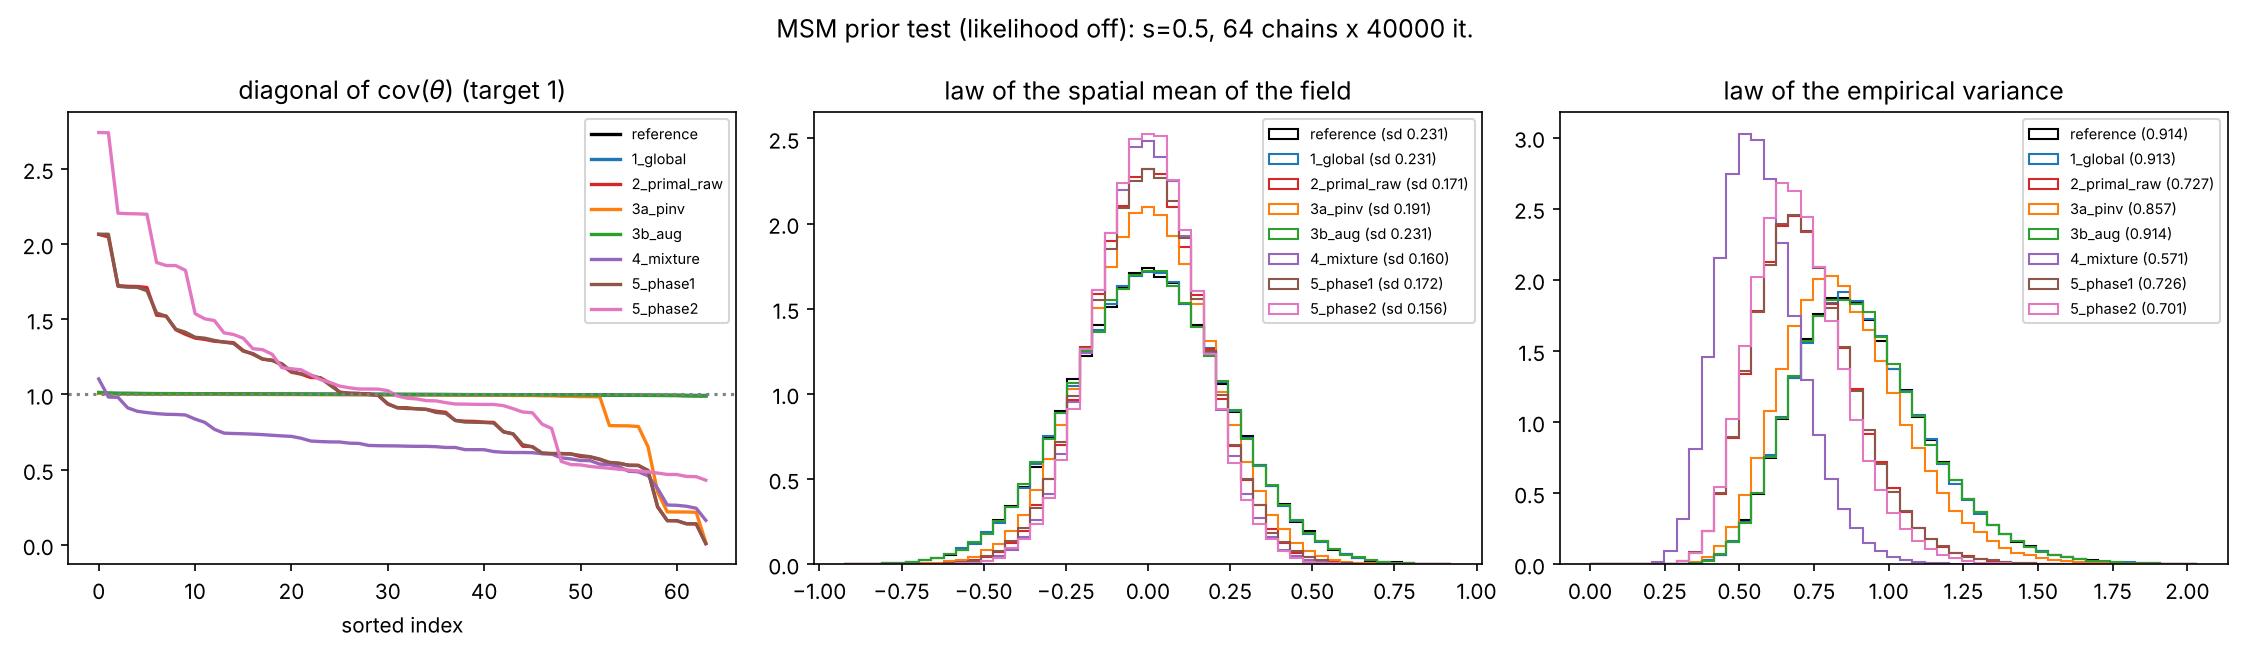
\includegraphics[width=\textwidth]{figures/msm_prior_test/fig_msm_prior_test.png}
\caption{Prior test: variances of $\theta_i$, law of the spatial mean, law of the empirical field variance.}\end{figure}

\section{Production results}
\subsection{Adaptation, misfit and mixing}
\begin{center}\small
\resizebox{\textwidth}{!}{\begin{tabular}{@{}lccccrr@{}}\toprule
 & final $s$ & mean AR & median $\rel$ & MPSRF($\theta$) & MPSRF($c$) & $<1.2$ at it.\\ \midrule
1 & 0.041 & 0.254 & 0.0205 & 1.127 & --- & 72\,023\\
2 & 0.051 & 0.253 & 0.0204 & 1.078$^\ast$ & 1.096 & 44\,473\\
3a & 0.041 & 0.253 & 0.0204 & 1.094$^\ast$ & 1.109 & 59\,144\\
3b & 0.041 & 0.262 & 0.0205 & 1.120 & 1.138$^\dagger$ & 68\,506\\
4 & 0.001 / 0.041 & 0.002 / 0.249 & 0.0332 & 1.611 & 1.568 / 1.828 & never\\
5 ph.\,1 & 0.051 & 0.253 & 0.0204 & 1.169$^\ast$ & 1.205 & 44\,473\\
5 ph.\,2 & 0.051--0.064 & 0.265 & 0.0207 & 1.165 & 1.297 & 90\,958\\
5 full run & & & & 1.075 & & 44\,432\\ \bottomrule
\end{tabular}}\end{center}
{\footnotesize $^\ast$ in the 58 range coordinates $V_+^\top\theta$ (the $\theta$ of these runs lies in a 58-dimensional subspace, so the 64-dimensional within-chain covariance is singular); $^\dagger$ joint $(c,\zeta)$, 70 dimensions. Experiment 4: primal / dual; MPSRF of the two projections $\Pi_p\theta$ / $\Pi_d\theta$. MPSRF uses the MATLAB-convention curve of \texttt{brho/mpsrf.py} (skip 2, step 15, burn 10) on the 900 saved samples per chain after $M$ (400 per phase for 5); the last column is the first crossing of 1.2.}

\medskip
\textbf{Acceptance and step sizes.} Adaptation reaches the 25\% target everywhere except the primal move of experiment 4 (Fig.~\ref{fig:ar4}). \textbf{Misfit.} Every healthy sampler has median $\rel\approx0.0204$ after adaptation (traces shown for 1 and 5 in Fig.~\ref{fig:rel}), i.e.\ $\Phi\approx\tfrac12(0.0204/0.003)^2\approx23$ (measured median $23.6$ before the switch in 5). This is $\approx6.4\times$ the data noise (0.0032) and is the expected posterior level for this problem; the traces show no drift after $M$. \textbf{Mixing.} $\theta$-MPSRF is between 1.08 and 1.13 for 1--3b (the global control is highest, 1.127), all below 1.2; experiment 5's phase-wise values (1.17, 1.17 from 400 samples each) and the local coefficients of phase 2 ($1.30$) are less settled simply because the windows are shorter.
\begin{figure}[h]\centering
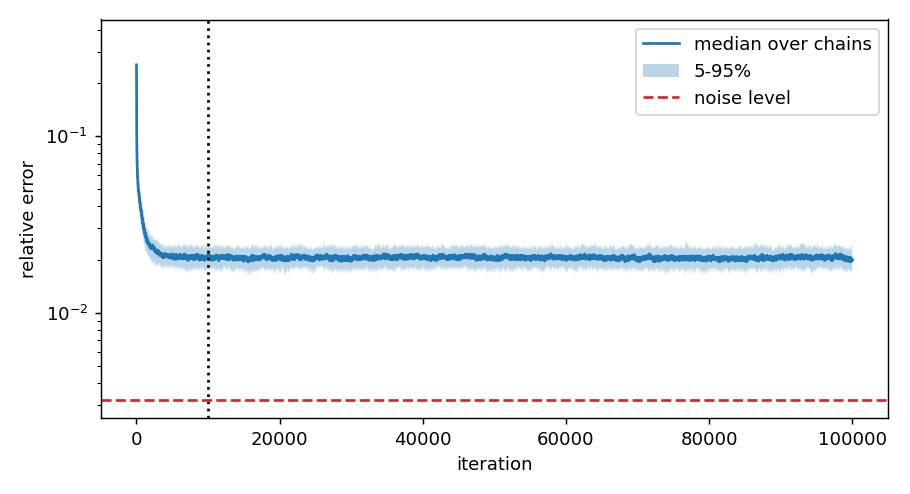
\includegraphics[width=.49\textwidth]{exp1_global/post/relerr_traces.png}\hfill
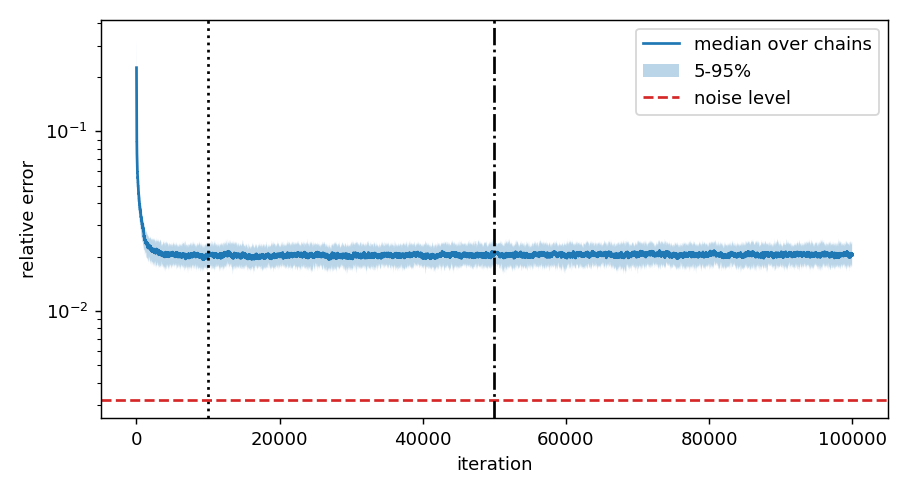
\includegraphics[width=.49\textwidth]{exp5_sequence/post/relerr_traces.png}
\caption{Relative error, median and 5--95\% band over 64 chains. Left: experiment 1. Right: experiment 5 (dotted: end of adaptation; dash-dotted: primal$\to$dual switch). Dashed red: realised noise level.}\label{fig:rel}\end{figure}

\subsection{Experiment 5: the primal$\to$dual switch}
Projecting each chain's final global field onto the dual basis changes $\Phi$ from $23.57$ to $24.80$ (median over chains) and $\rel$ from $0.0206$ to $0.0211$: a small step that is not visible at the scale of Fig.~\ref{fig:rel}. Both phases then run at the 25\% acceptance level with unchanged relative error.

\subsection{Experiment 4: why it fails}
The primal move proposes $\theta'=B_p\,(\sqrt{1-s^2}\,\Pi_p\theta+s\xi)$. Even at $s=0$ this is the lossy round trip $\theta\mapsto B_p\Pi_p\theta$, which changes the field by $19\%$ (relative $L_2$, prior draws; dual: $5.7\%$). Against a likelihood this sharp (the chains sit at $\rel=0.02$ and $\sigma_{rel}=0.003$), such proposals are almost always rejected: the adapter drives $s$ to its floor $10^{-3}$ without lifting acceptance (mean $0.16\%$, Fig.~\ref{fig:ar4}). Effectively only the dual move works, with $\approx$ half the iterations wasted and a round trip that is itself lossy. The chains plateau at $\rel=0.033$, MPSRF is $1.6$ (no crossing of 1.2), and the pointwise sd of $\log\kappa$ is $0.22$, so the result is a non-converged, biased sampler rather than a posterior. The mechanism (round-trip field change) is inferred from prior draws and the acceptance data, not measured at posterior states.
\begin{figure}[h]\centering
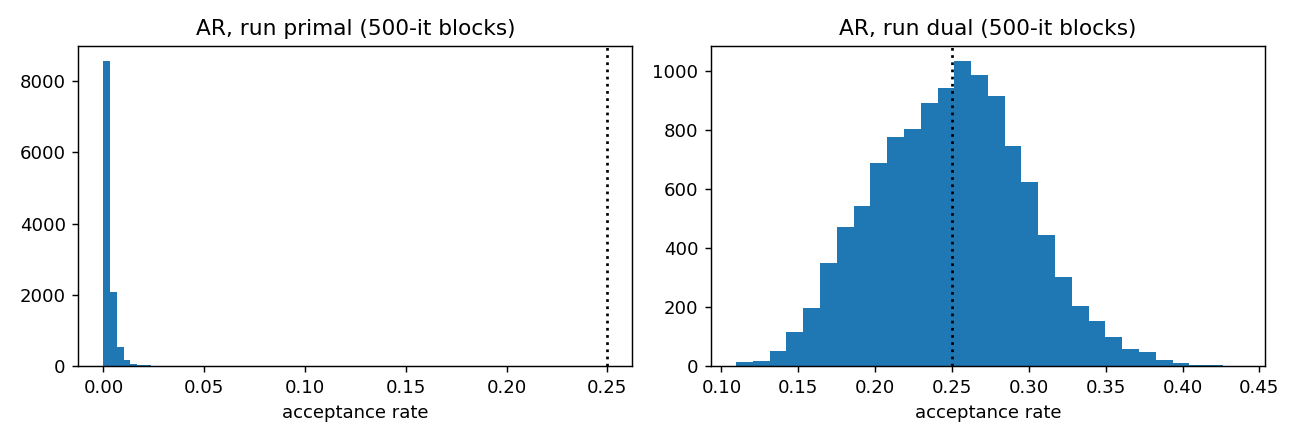
\includegraphics[width=.8\textwidth]{exp4_mixture/post/ar_hist.png}
\caption{Experiment 4 acceptance rate (500-iteration blocks, 64 chains) for the primal (left) and dual (right) moves.}\label{fig:ar4}\end{figure}

\subsection{Posterior fields}
Pointwise mean and sd from 5\,000 post-$M$ samples per experiment (2\,500 per phase for 5).
\begin{center}\small
\resizebox{\textwidth}{!}{\begin{tabular}{@{}lrrrr@{}}\toprule
 & mean sd $\log\kappa$ & ratio to exp.\,1 & mean sd $p$ & rms(mean $\log\kappa-$truth)\\ \midrule
1 global & 0.570 & 1.00 & 0.0094 & 0.415\\
2 primal raw & 0.473 & 0.83 & 0.0091 & 0.495\\
3a pseudo-inverse & 0.511 & 0.90 & 0.0092 & 0.456\\
3b null-space term & 0.575 & 1.01 & 0.0093 & 0.411\\
4 mixture & 0.217 & 0.38 & 0.0063 & 0.556\\
5 (phase 1 / 2 / pooled) & 0.468 / 0.472 / 0.492 & 0.82 / 0.83 / 0.86 & 0.0091 / 0.0094 / 0.0094 & 0.495 / 0.437 / 0.445\\ \bottomrule
\end{tabular}}\end{center}
The sd of $\log\kappa$ orders the samplers as the prior test predicts: $3b\approx1>3a>5\approx2\gg4$. The pressure sd, which is constrained by the data, differs by about $3\%$ at most among 1--3b and 5. The posterior mean of $\log\kappa$ is closest to the truth for 3b and 1 (rms $0.41$) and farthest for 2 and 4. The raw samplers' narrower posteriors do not buy a better mean, they also fit the truth worse.
\begin{figure}[h]\centering
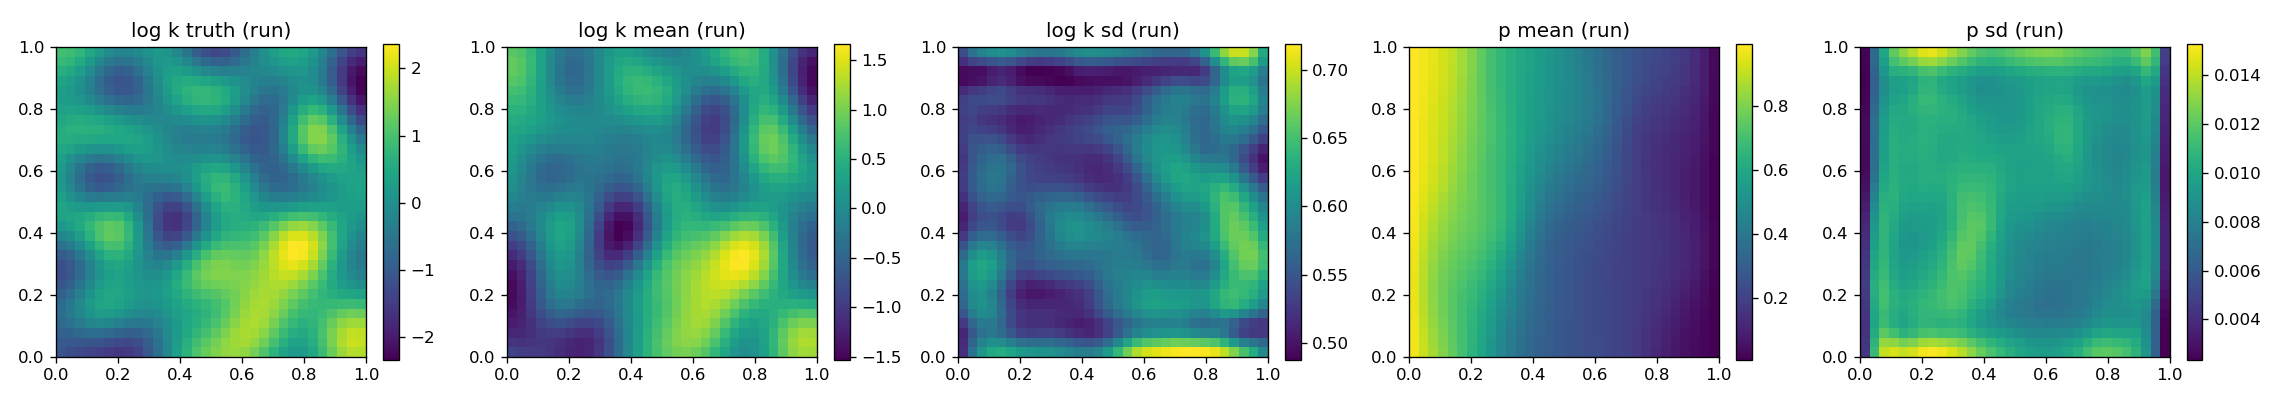
\includegraphics[width=\textwidth]{exp1_global/post/fields_run.png}\\[2pt]
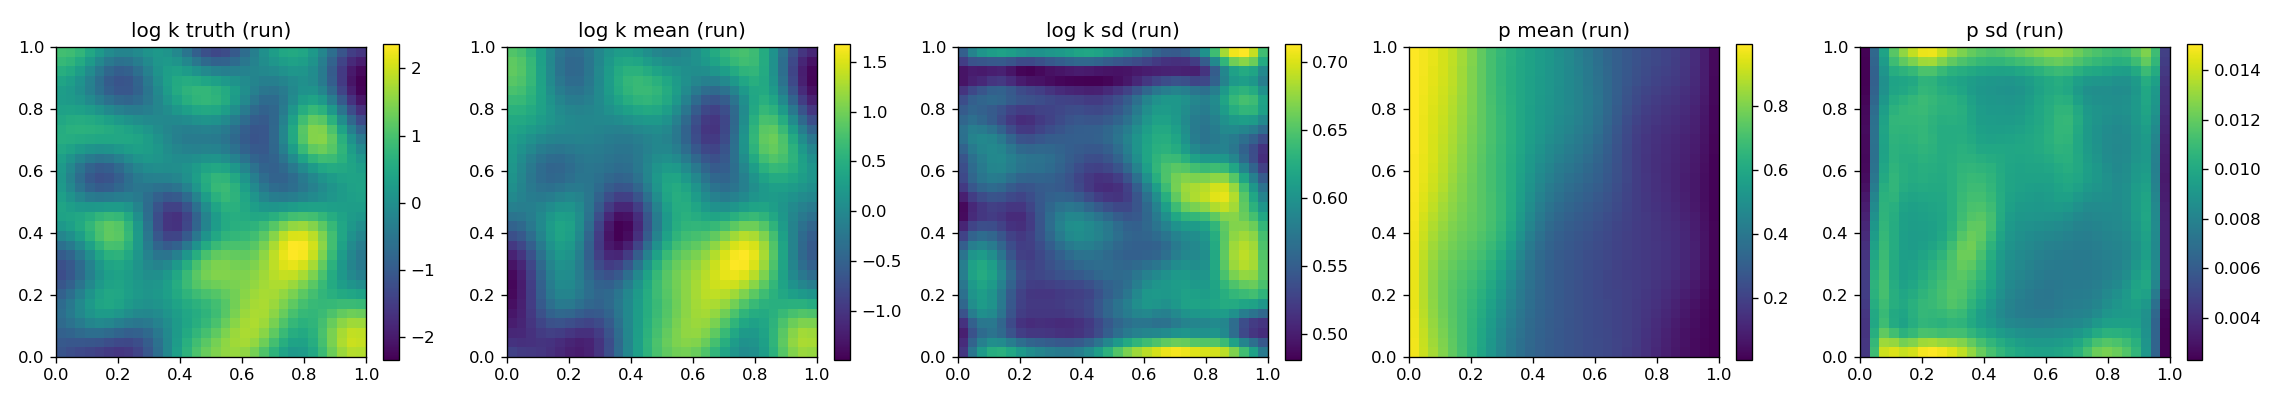
\includegraphics[width=\textwidth]{exp3b_primal_aug/post/fields_run.png}\\[2pt]
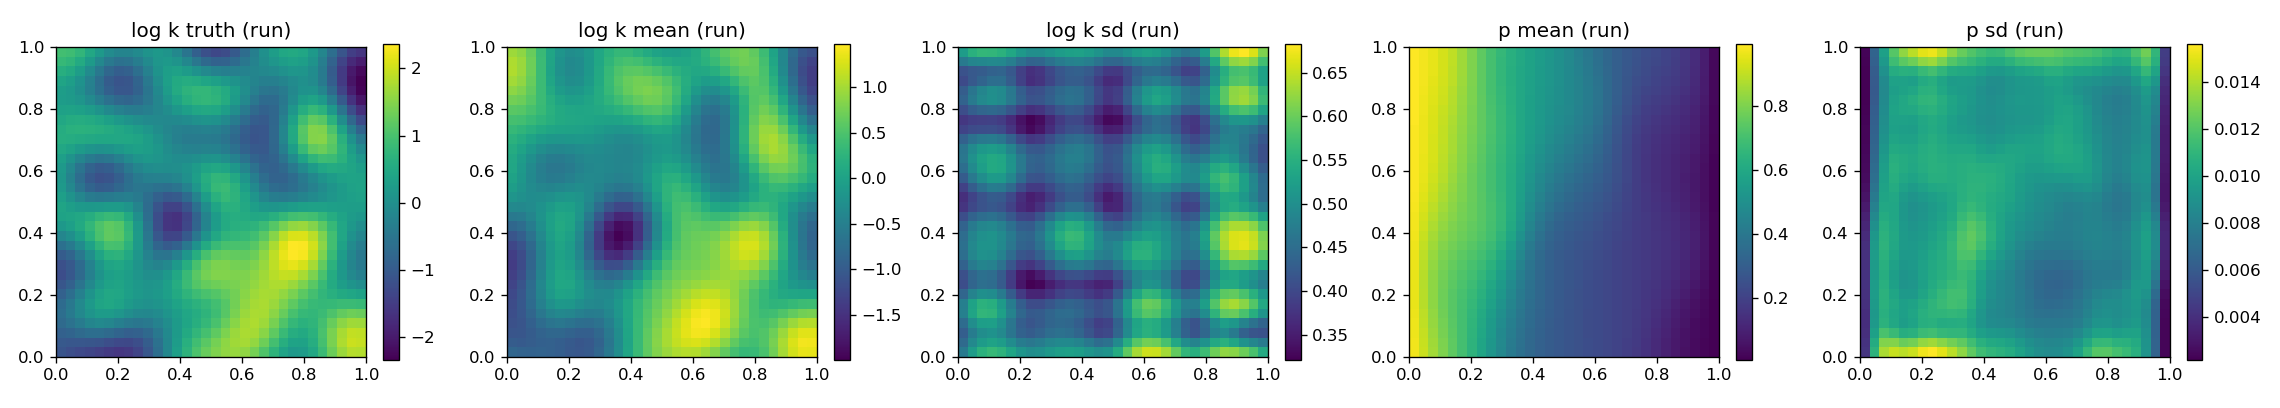
\includegraphics[width=\textwidth]{exp2_primal_raw/post/fields_run.png}\\[2pt]
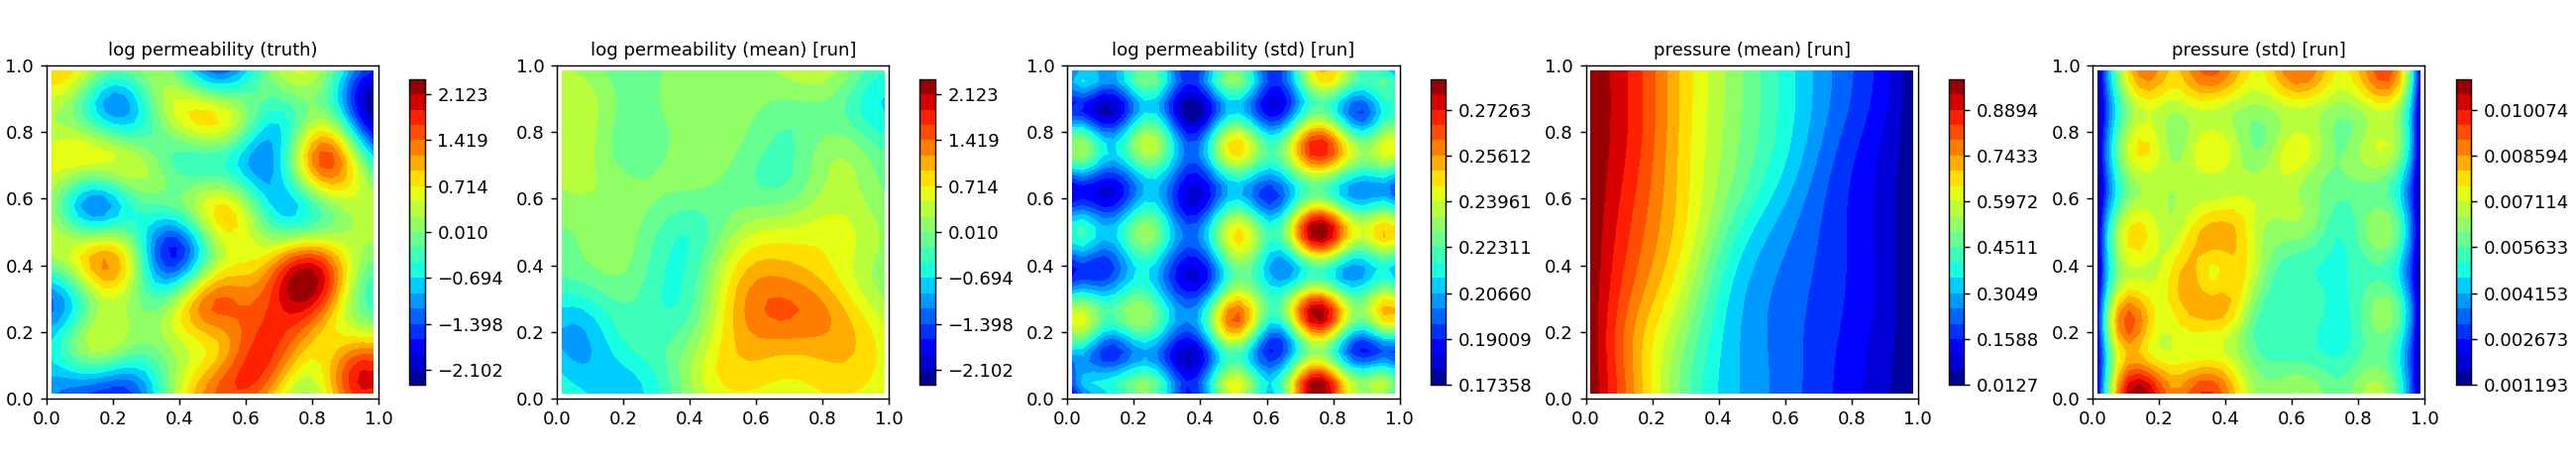
\includegraphics[width=\textwidth]{exp4_mixture/post/fields_run.png}
\caption{Truth, posterior mean and sd of $\log\kappa$, posterior mean and sd of the pressure, for experiments 1, 3b, 2 and 4 (top to bottom). Each panel has its own color scale. These are the first-run figures (default colormap); the group-style contour plots are regenerated by \texttt{run\_msm\_post.py} (Section~\ref{sec:repro}).}\end{figure}

\section{Interpretation}
\begin{itemize}
\item The six-direction rank deficit of the primal $\Sigma_{ms}$ is the whole difference between 3a and 3b: with the null-space term the whitened primal sampler is exactly global pCN; without it the sampler cannot move along six directions and the posterior is slightly too narrow (sd $0.90\times$, and the prior test gives $0.93$ in variance).
\item Raw primal sampling (2) targets the wrong prior, $N(0,\Sigma_{ms})$ whose per-coordinate prior variances range from $0.01$ to $2.1$ (prior test). It is nevertheless as fast as the others per iteration and acceptance, so it gains little in mixing (MPSRF 1.08 vs.\ 1.13; no uncertainty on that difference is available), and the price is $17\%$ less posterior spread and a worse posterior mean.
\item Experiment 5 inherits raw primal's variance deficit (and the dual's, $0.75$ in the prior test) but loses little at the switch; the full-run $\theta$ MPSRF of $1.075$ includes both phases.
\item Experiment 4 shows that alternating with a lossy projection of a \emph{state} is not a substitute for proposing in the local coefficients (experiments 2 and 5): the projection error enters every proposal.
\end{itemize}

\section{Caveats}\label{sec:caveats}
\begin{itemize}
\item One data set and one set of chain seeds. The 10--17\% differences in posterior sd (2, 3a, 5 vs.\ 1) are consistent across the prior test and production but have no repeated-data or bootstrap uncertainty here.
\item The MPSRF values in this report use the first-pass convention (window starting after the adaptation period, samples saved every 100 iterations); the group's convention (window starting at iteration 1\,000, adaptation included) and 50-iteration saving are implemented in \texttt{run\_msm\_post.py} but the numbers have not been recomputed here. \item MPSRF is 1.08--1.14, not below 1.05; sd estimates from 64 chains of 900 saved samples are themselves uncertain by an amount not quantified here. For 2, 3a and phase 1 of 5 it is computed in range coordinates, so values are not directly comparable in dimension (58 vs.\ 64).
\item The likelihood is a global-norm relative likelihood with $\sigma_{rel}=0.003$ and data noise equal to it; the plateau at $\rel=0.020$ (about $6.4\times$ the noise) means the posterior is dominated by what the 64 parameters and the likelihood weight allow, not by the noise floor. With a tempered likelihood (as in the repo's earlier runs, $\sigma_{rel}=\varepsilon/\sqrt{n_{\rm eff}}$) the picture could differ.
\item Experiment 4's failure mechanism is inferred, not measured at posterior states.
\item Field figures here are not in the final plotting style (below).
\end{itemize}

\section{Reproduction and next steps}\label{sec:repro}
Code: \texttt{brho/msm\_local.py}, \texttt{brho/msm\_sampler.py}, \texttt{experiments/run\_msm\_chains.py}, \texttt{run\_msm\_post.py}, \texttt{run\_msm\_compare.py}; six \texttt{cluster/slurm/msm\_exp*.sbatch}; spec \texttt{docs/msm\_local\_kle\_experiment.md}; outputs \texttt{runs/msm\_local\_kle\_2026-11/}.

\textbf{Field plots.} \texttt{experiments/msm\_fieldplots.py} draws filled contours with \texttt{jet} (colormaps for fields and sd maps are separate defaults, \texttt{CMAP\_MAIN}, \texttt{CMAP\_STD}, 20 levels; \texttt{--cmap}, \texttt{--cmap-std}, \texttt{--levels} on the command line). The posterior field arrays are now saved to \texttt{post/fields.npz} and kept in git, so after one rerun of \texttt{run\_msm\_post.py} on the cluster per experiment, \texttt{--replot-only} redraws any style without the chains, and \texttt{run\_msm\_compare.py} produces six-panel sd/mean maps on shared scales and a table.

\textbf{Suggested next steps.} (i) Regenerate the fields in the chosen style and add the six-panel comparison; (ii) repeat with a second truth seed to put an error bar on the sd ratios; (iii) if experiment 4 is to be kept, propose in the local coefficients of a persistent state, or restrict it to the dual grid; (iv) decide whether the primal grid should use 6 local modes per block, which makes $\Sigma_{ms}$ full rank (as a separate study).
\end{document}
